\documentclass[12pt]{article}
 
\usepackage[margin=1in]{geometry} 
\usepackage{amsmath,amsthm,amssymb}
\usepackage[spanish]{babel}
\usepackage[utf8]{inputenc}
\usepackage{tikz-cd}
\usepackage{amsmath}
\usepackage[shortlabels]{enumitem}
\usepackage{mathtools}

% cosas entre comillas 
\usepackage{csquotes}

\usepackage{tikz}
\usepackage{booktabs}
\usepackage{multirow}
\usepackage{siunitx}

\decimalpoint
\usepackage{xcolor}

\usepackage{personalcommands}
\newcommand{\flechita}[1]{\overset{\rightarrow}{ #1 }}
\newtheorem{theorem}{Teorema}[section]
\newtheorem{lemma}[theorem]{Lema}
\newtheorem{prop}[theorem]{Proposición}
\newtheorem{coro}[theorem]{Corolario}
\newtheorem{conj}[theorem]{Conjetura}
\newtheorem{ejercicio}{Ejercicio}
\newtheorem*{ejercicio*}{Ejercicio}
\theoremstyle{definition}
\newtheorem{definition}[theorem]{Definición}
\newtheorem{example}[theorem]{Ejemplo}
\theoremstyle{remark}
\newtheorem{remark}[theorem]{Nota}
\newtheorem{notacion}[theorem]{Notación}
\newcommand{\continuas}[1][]{C^{ #1 }[a,b]}
\newcommand{\continuasabierto}[1][]{C^{ #1 }(a,b)}
\newcommand{\soportecompacto}{\mathcal{D}(a,b)}
\newcommand{\xcero}{(a,b)}
\newcommand{\xcerocerrado}{[a,b]}
\newcommand{\fvariaciones}{F(x,y(x),y'(x))}
\usepackage{float}

\begin{document}

\textbf{Ejercicio 3.} Disponemos de una red con la topología mostrada en la figura. Usando direcciones IPv4 de clase C pública, realice una asignación de direcciones, en la que todas las subredes deben tener la máscara /27 y además ser contiguas.
\begin{itemize}
\item Asigne direcciones de red a todas las redes de la figura.
\item Asigne direcciones IP a todos los interfaces que corresponda.
\item Asigne el default Gateway (puerta de enlace predeterminada) a todos los PCs.
\item Escriba las rutas estáticas en la tabla de enrutamiento del router \textit{RoutC} para poder llegar a todas las redes por el camino más corto. Incluya en cada entrada $<$red destino$>$ $<$máscara$>$ $<$next hop$>$.
\end{itemize}

\begin{figure}[H]
   \center
  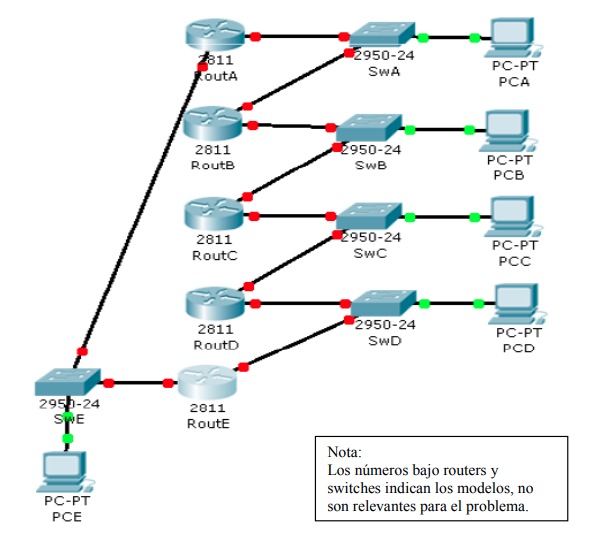
\includegraphics[scale=0.5]{img/3.png}
\end{figure}

\newpage

Primero se detectan la diferentes redes del sistema y se asigna que interfaces FastEthernet  van a ser usadas.

\begin{figure}[H]
   \center
  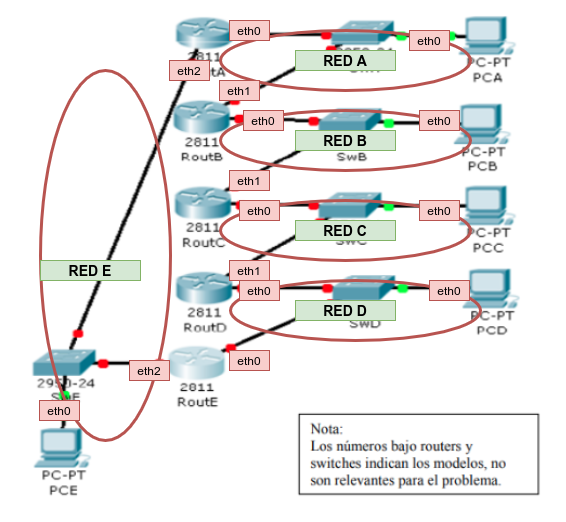
\includegraphics[scale=0.5]{img/2.png}
\end{figure}

Para asignar las subredes, se van a usar las direcciones empezando por $216.216.0.0$. Como hay que fijar máscara /27, los últimos 5 bits hay que dejarlos para los hosts. Además, para asignarlas de forma contigua, se suma 1 (binario) el tercer bit del último octeto:

\begin{center}
\begin{tabular}{|c|c|c|}
\hline 
Red & Dirección & Interfaz \\ 
\hline 
A &  216.216.0.32 & --- \\ 
\hline 
B &  216.216.0.64 & --- \\ 
\hline 
C &  216.216.0.96 & --- \\ 
\hline 
D &  216.216.0.128 & --- \\ 
\hline 
E  &  216.216.0.160 & --- \\ 
\hline 
\end{tabular} 
\end{center}

Lo siguiente es asignarle direcciones a las interfaces de los routers de cada subred:

\begin{center}
\begin{tabular}{|c|c|c|}
\hline 
Router & Interfaz & Dirección \\ 
\hline 
\multirow{2}{*}{RoutA} & eth0 & 216.216.0.33 \\ 
  & eth2 & 216.216.0.161 \\ 
\hline 
\multirow{2}{*}{RoutB} & eth0 & 216.216.0.65 \\ 
 & eth1 & 216.216.0.34 \\ 
\hline 
\multirow{2}{*}{RoutC} & eth0 & 216.216.0.97 \\ 
 & eth1 & 216.216.0.66 \\ 
\hline 
\multirow{2}{*}{RoutD} & eth0 & 216.216.0.129 \\ 
 & eth1 & 216.216.0.98 \\ 
\hline 
\multirow{2}{*}{RoutE} & eth0 & 216.216.0.130 \\ 
 & eth2 & 216.216.0.162 \\ 
\hline 
\end{tabular} 
\end{center}

Ahora se le asigna a cada host una IP, como ya se han usado dos para cada router en cada subred, y solo hay un host por red, simplemente hay que añadir 3 a la dirección de red para obtener la IP de cada host:

\begin{center}
\begin{tabular}{|c|c|c|}
\hline 
Host & Dirección IP & Interfaz \\ 
\hline 
PCA &  216.216.0.35 & eth0 \\ 
\hline 
PCB & 216.216.0.67  & eth0 \\ 
\hline 
PCC &  216.216.0.99  & eth0\\ 
\hline 
PCD & 216.216.0.131   & eth0\\ 
\hline 
PCE & 216.216.0.163  & eth0 \\ 
\hline 
\end{tabular}
\end{center}

Una vez que todas las redes y hosts tienen sus respectivas IPs, se puede completar la tabla de enrutamiento del RouterC:

\begin{center}
\begin{tabular}{|c|c|c|c|}
\hline 
  & destino & máscara & next hop \\ 
\hline 
S & RED A & 255.255.255.224  &  216.216.0.65 \\ 
\hline 
C & RED B & 255.255.255.224  &  - \\ 
\hline 
C & RED C & 255.255.255.224  &  -  \\ 
\hline 
C & RED D & 255.255.255.224  &  216.216.0.98 \\ 
\hline 
C & RED E & 255.255.255.224  &  216.216.0.98 \\ 
\hline 
S & default & 0.0.0.0 & 216.216.0.65 \\ 
\hline 
\end{tabular}
\end{center}

La tabla de enrutamiento sale bastante sencilla porque todos los routers están conectados en un \textit{círculo}, luego para alcanzar las redes que no se encuentran directamente conectadas simplemente hay que pasar el paquete \textit{hacia arriba} o \textit{hacia abajo}, según sea más corto.


\newpage

\textbf{Ejercicio 4.} Los routers $Rx\_A$ y $Rx\_B$ de la figura están configurados para ejecutar \textbf{NAT dinámico Overload} de manera que las direcciones \textit{Inside local} en las redes $A$ y $B$ sean transformadas a un único \textit{Inside global} que coincide con la IP de su interfaz F0/1 respectivo. Tanto $Rx\_A$ como $Rx\_B$ saben como llegar a las redes $A$ y $B$ mediante \textbf{rutas estáticas} con next-hop la IP del F0/1 del siguiente router. Cada router del lado INSIDE, R1 y R2, tiene configurada una ruta por defecto a través del F0/0 de $Rx\_A$ y $Rx\_B$ respectivamente.
\begin{figure}[H]
   \center
  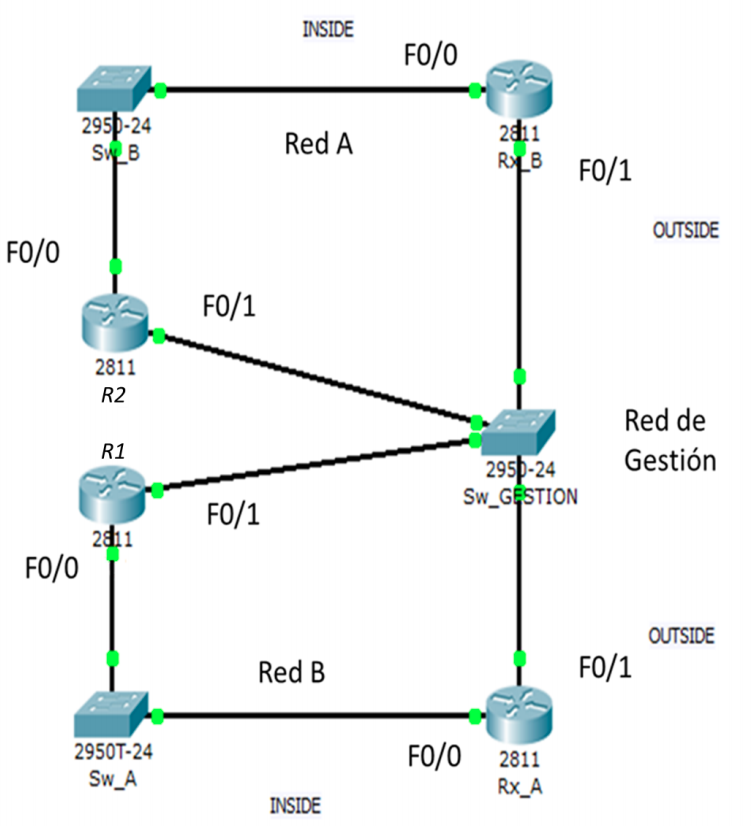
\includegraphics[scale=0.25]{img/4.png}
\end{figure}
\begin{enumerate}[(a)]
\item Asigne direcciones IP y máscaras a todos los interfaces que considere.

Como sólo se va a hacer \textit{ping} al router \textit{R2}, es suficiente con asignar IPs en la red de gestión, cuya dirección será 172.16.0.0/24. A la interfaz \textit{F0/1} del router \textit{Rx\_B} se le asigna la IP 172.16.0.1 (usada como inside global).

\item ¿Qué ocurriría si R1 hiciera ping a la dirección INSIDE GLOBAL de R2?

Si se hace ping a su INSIDE GLOBAL, es decir, a 172.16.0.1, todo funcionará correctamente porque los paquetes del  ping saben ir y volver del router \textit{R1} a \textit{Rx\_B}

\item ¿Y si R1 hiciera ping a la dirección INSIDE LOCAL de R2?

Esta no va a funcionar ya que estamos usando la dirección INSIDE LOCAL. Ningún router sabe que hacer con esa dirección, porque solo tiene \textit{sentido} dentro de la red A. Cuando se haga el \textit{ping}, \textit{R1} no va a saber donde mandar esos paquetes, así que usará la opción default, es decir, \textit{Rx\_A}. Ese router tampoco sabe donde mandar esos paquetes, así que si tiene opción default los mandará a esa. Esto se va a repetir hasta que se alcancen los timeouts y se pierdan todos los paquetes.
\end{enumerate}


\end{document}